
\documentclass[journal]{IEEEtran}

\usepackage{amsfonts}
\usepackage{cite}
\usepackage{amsmath}
\usepackage{graphicx}
\usepackage{epstopdf}
\usepackage{amsthm}
\usepackage{color}


%supposed to center images
%\usepackage{floatrow}

%for multiline comments
\usepackage{verbatim}

%for arays
\usepackage{array}

%for matrices with labels
\usepackage{kbordermatrix}% http://www.hss.caltech.edu/~kcb/LaTeX.shtml

%the default image location
\graphicspath{{graph_stats/}{by_user/}{by_metric/}{all_metrics/}{muxViz/}}

% correct bad hyphenation here
\hyphenation{op-tical net-works semi-conduc-tor}

\begin{document}

\title{Student interactions on Facebook and in reality}



\author{A. Gajduk and
        L. Kocarev,~\IEEEmembership{Fellow,~IEEE}%
%\thanks{Copyright (c) 2012 IEEE. Personal use of this material is permitted. However, permission to use this material for any other purposes must be obtained from the IEEE by sending an email to pubs-permissions@ieee.org.}
%\thanks{A. Gajduk is with the Macedonian Academy of Sciences and Arts, Skopje, Macedonia. E-mail: agajduk@manu.edu.mk}

%\thanks{L. Kocarev is with the Macedonian Academy of Sciences and Arts, Skopje, Macedonia; the Faculty of Computer Sciences and Engineering, University ``Ss Cyril and Methodius'', Skopje, Macedonia and the BioCircuits Institute, UC San Diego, La Jolla, CA 92093-0402, USA. E-mail: lkocarev@ucsd.edu}
%\thanks{Digital Object Identifier:}
}

%
\maketitle
%

\begin{figure*}[!htb]
\centering
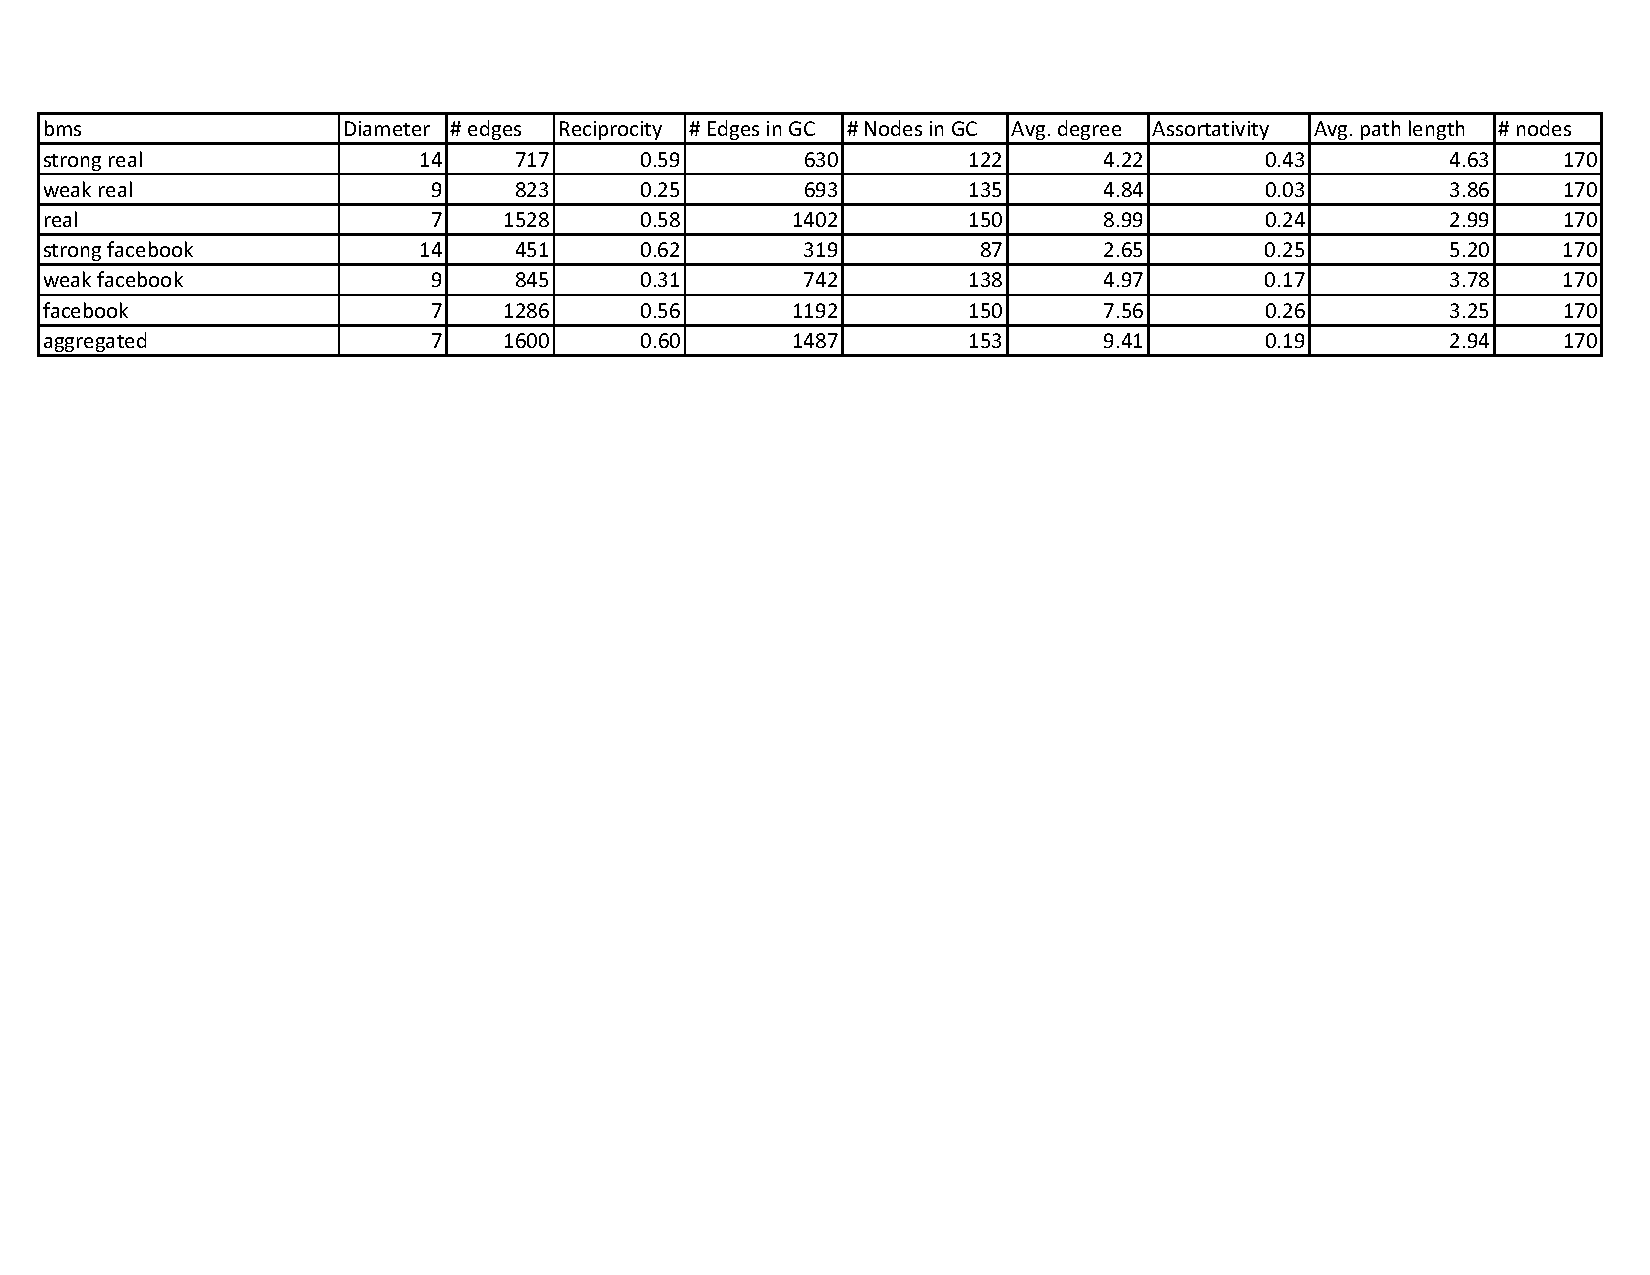
\includegraphics[scale=.65]{bms_stats.pdf}
\caption{Basic global graph statistics for BMS}
\end{figure*}

\begin{figure*}[!htb]
\centering
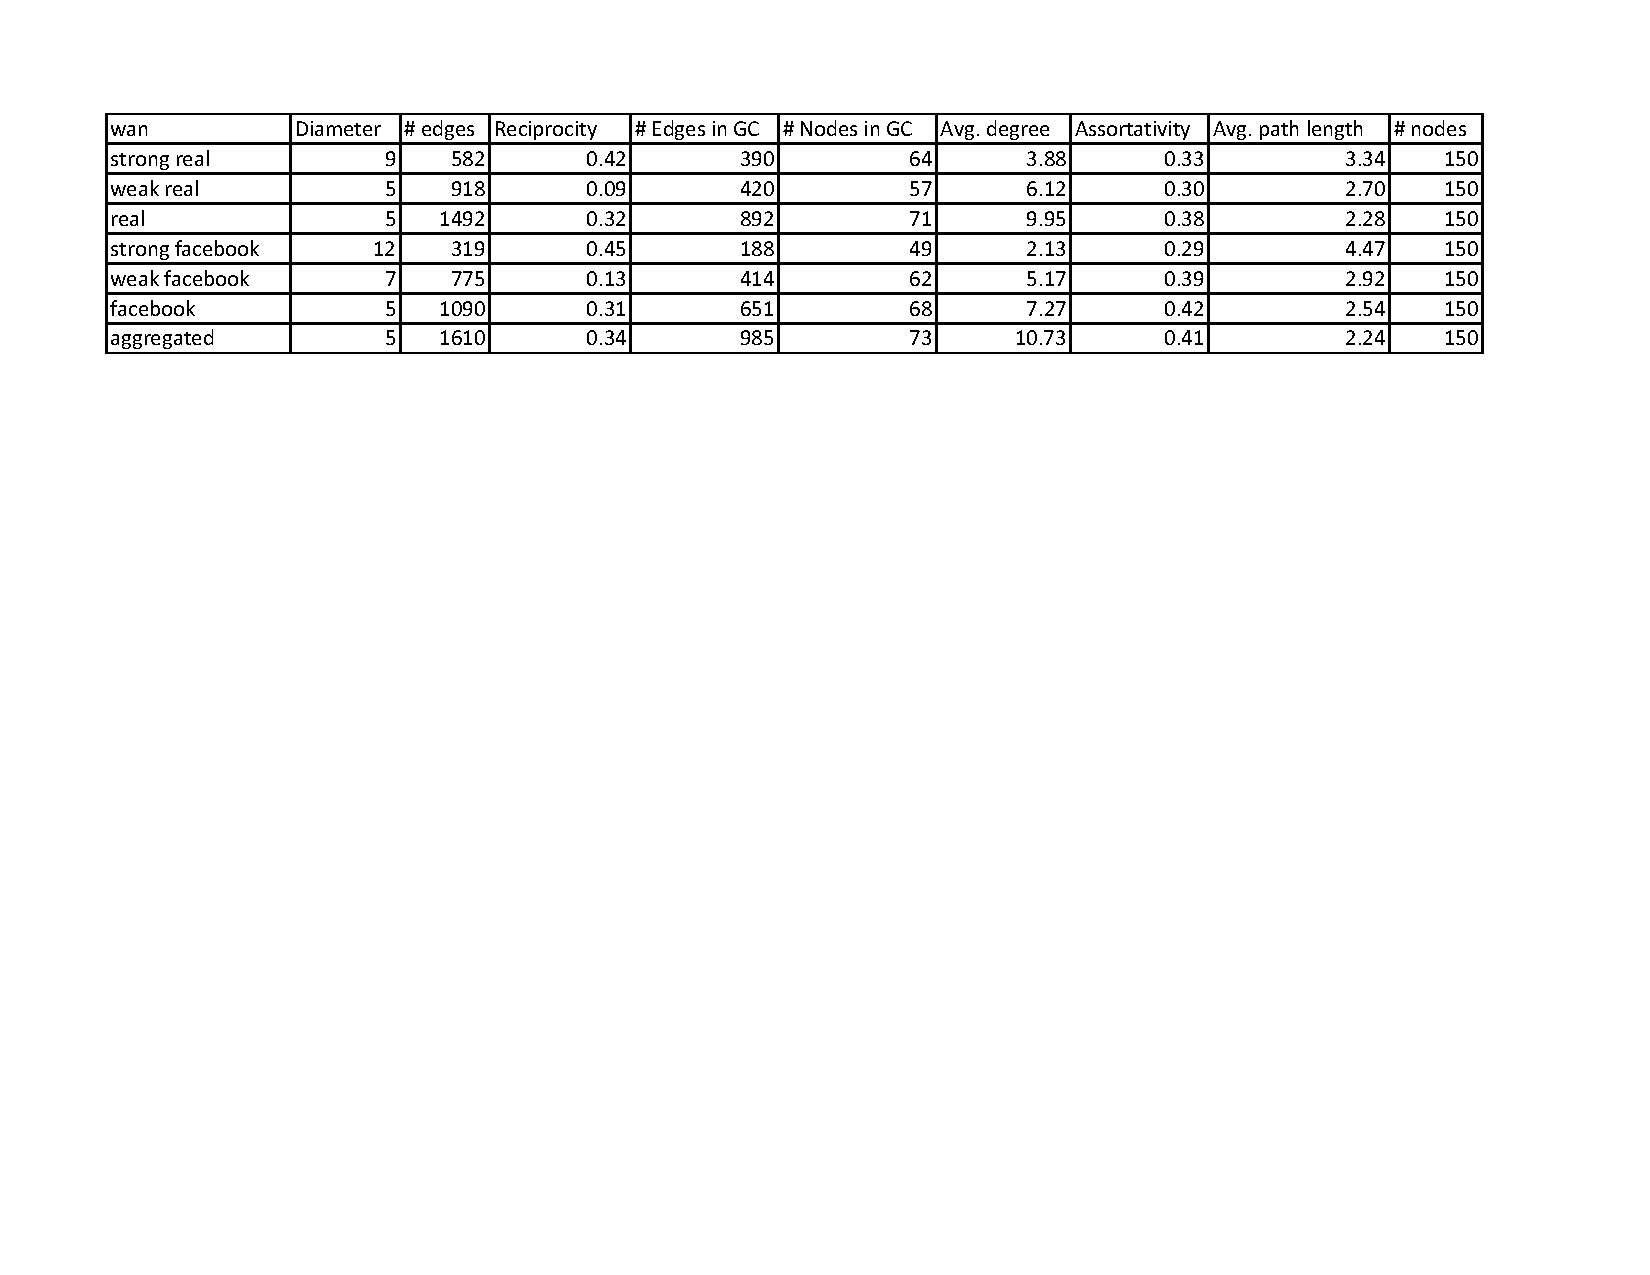
\includegraphics[scale=.75]{wan_stats.pdf}
\caption{Basic global graph statistics for WAN}
\end{figure*}

\begin{figure*}[!htb]
\centering
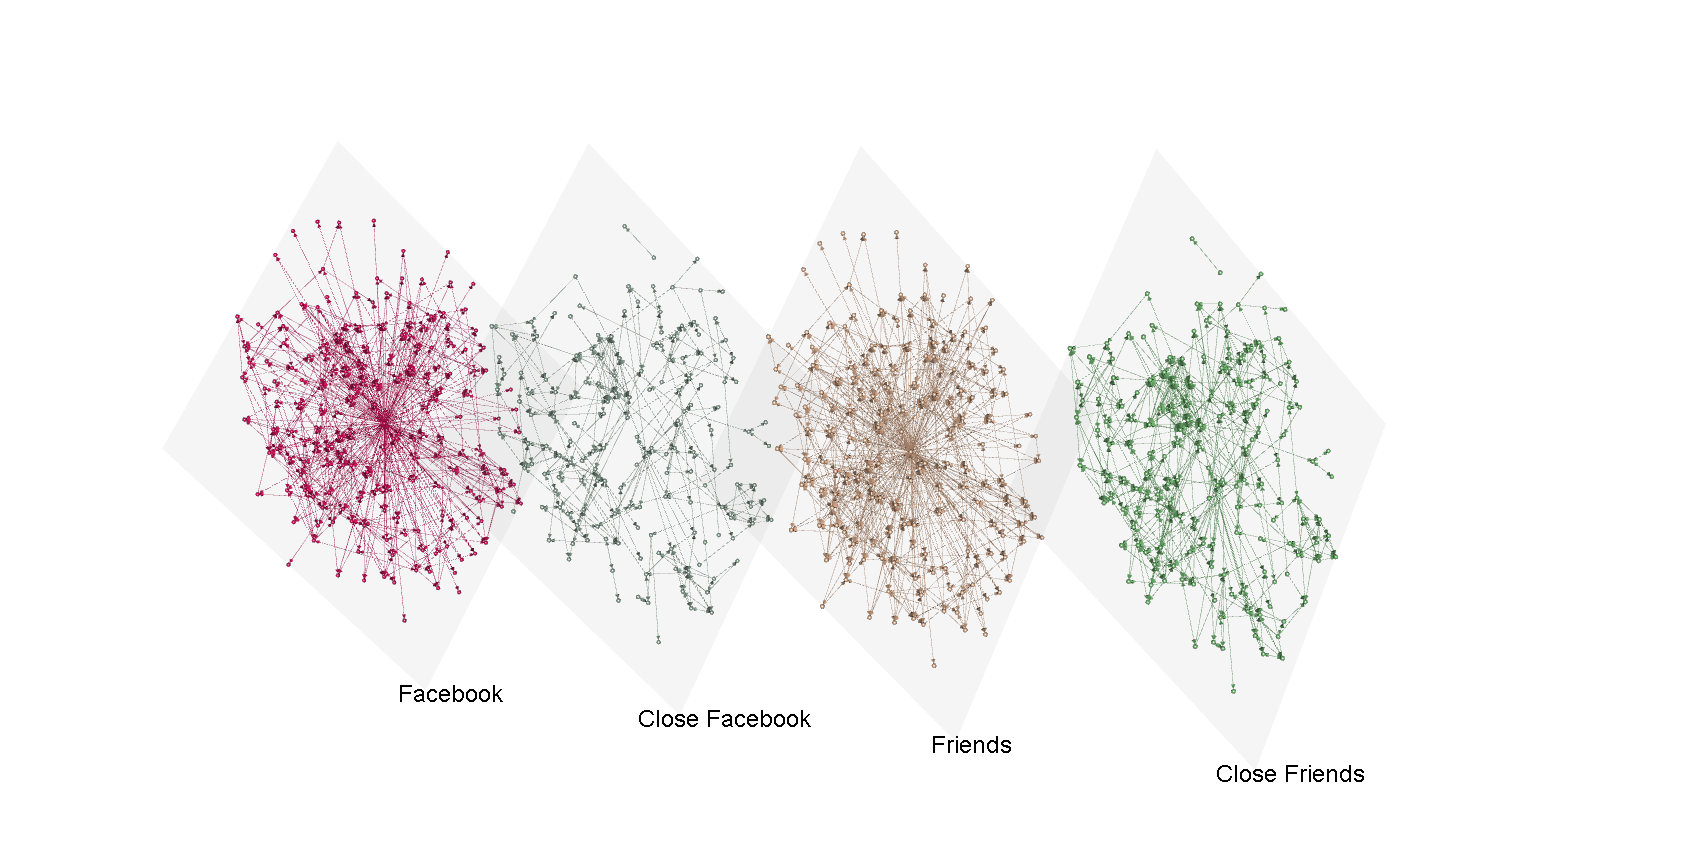
\includegraphics[scale=.3]{bms_frchterman}
\caption{Multilayer 3D visualization of BMS graphs in MuxViz}
\end{figure*}

\begin{figure*}[!htb]
\centering
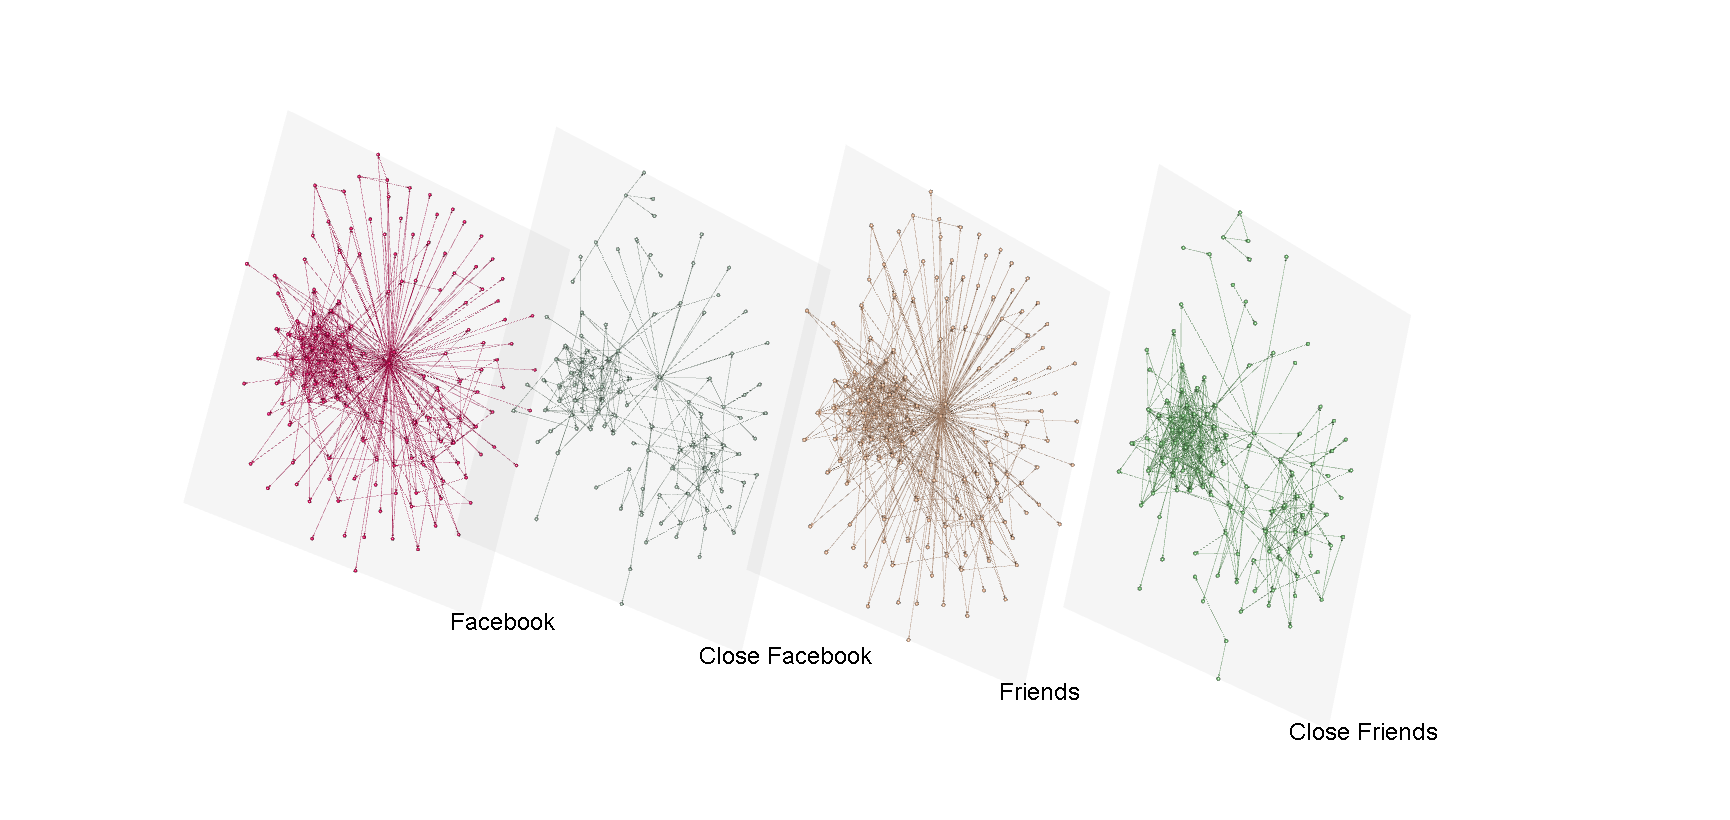
\includegraphics[scale=.29]{wan_bez15}
\caption{Multilayer 3D visualization of WAN graphs in MuxViz}
\end{figure*}

\begin{figure*}[!htb]
\centering
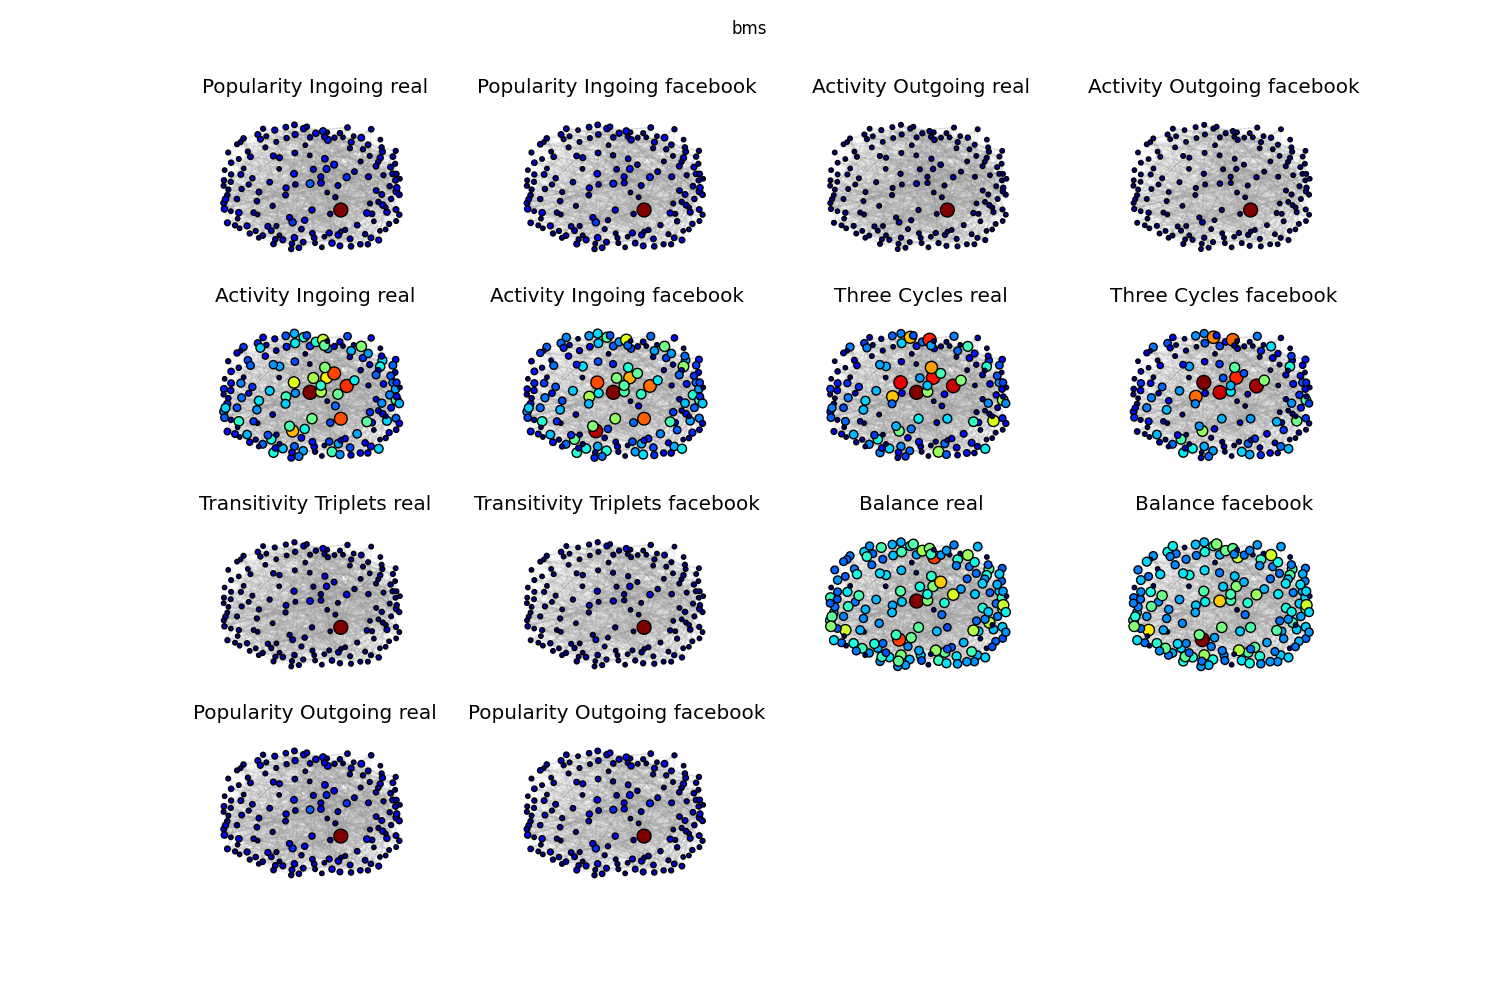
\includegraphics[scale=.55]{bms_both}
\caption{Real and facebook node metrics visualization for BMS}
\end{figure*}


\begin{figure*}[!htb]
\centering
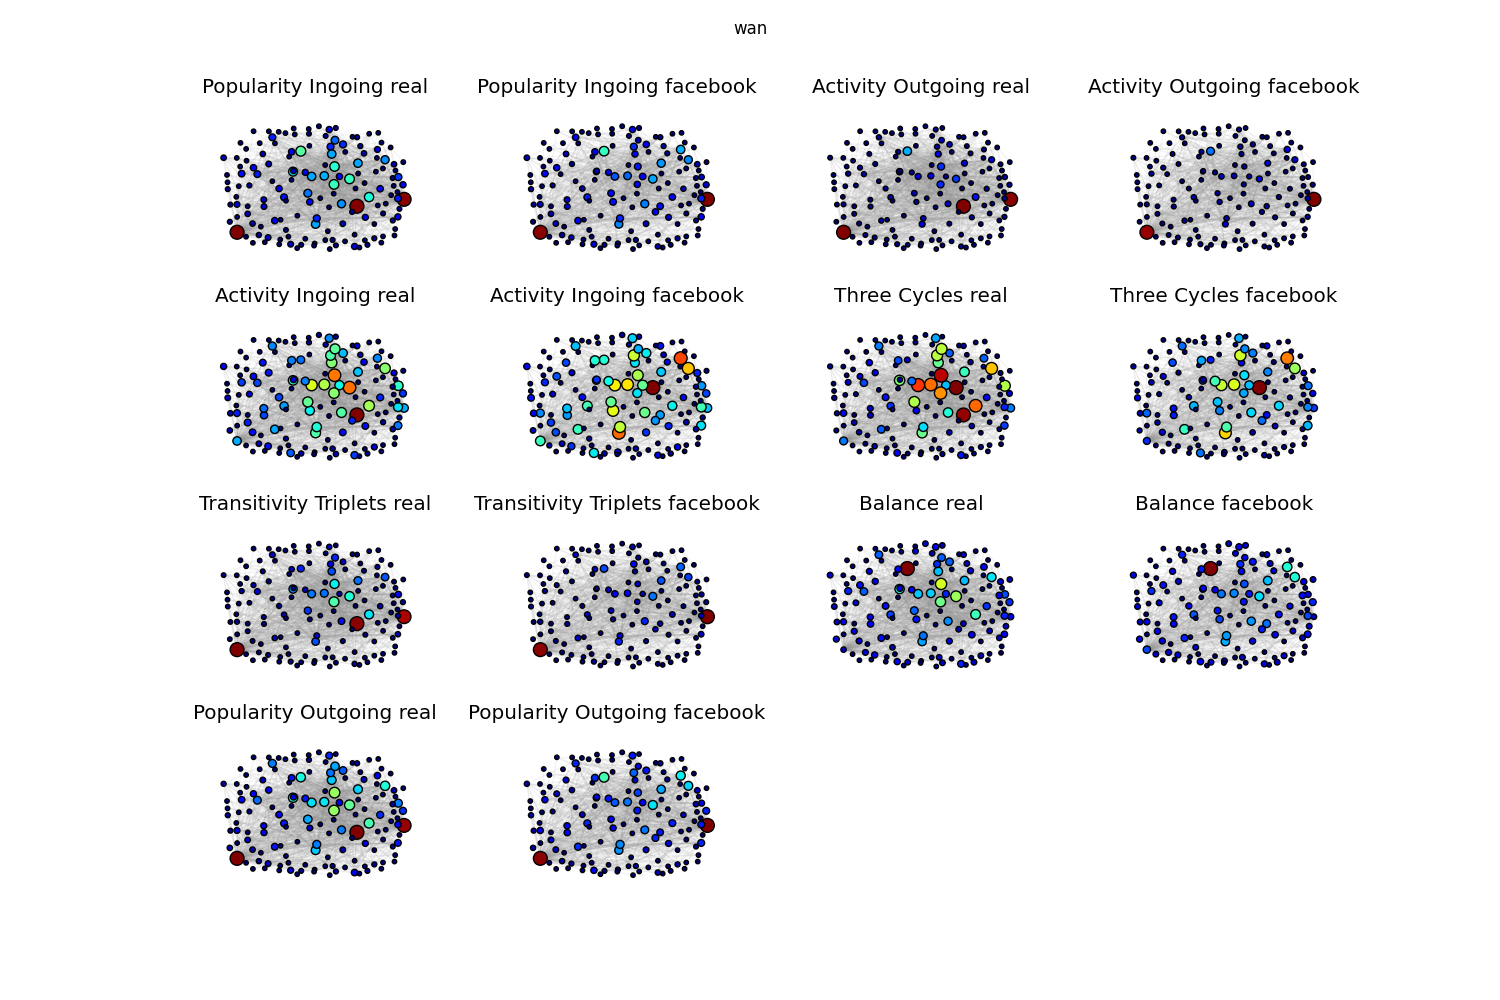
\includegraphics[scale=.55]{wan_both}
\caption{Real and facebook node metrics visualization for WAN}
\end{figure*}

\begin{figure*}[!htb]
\centering
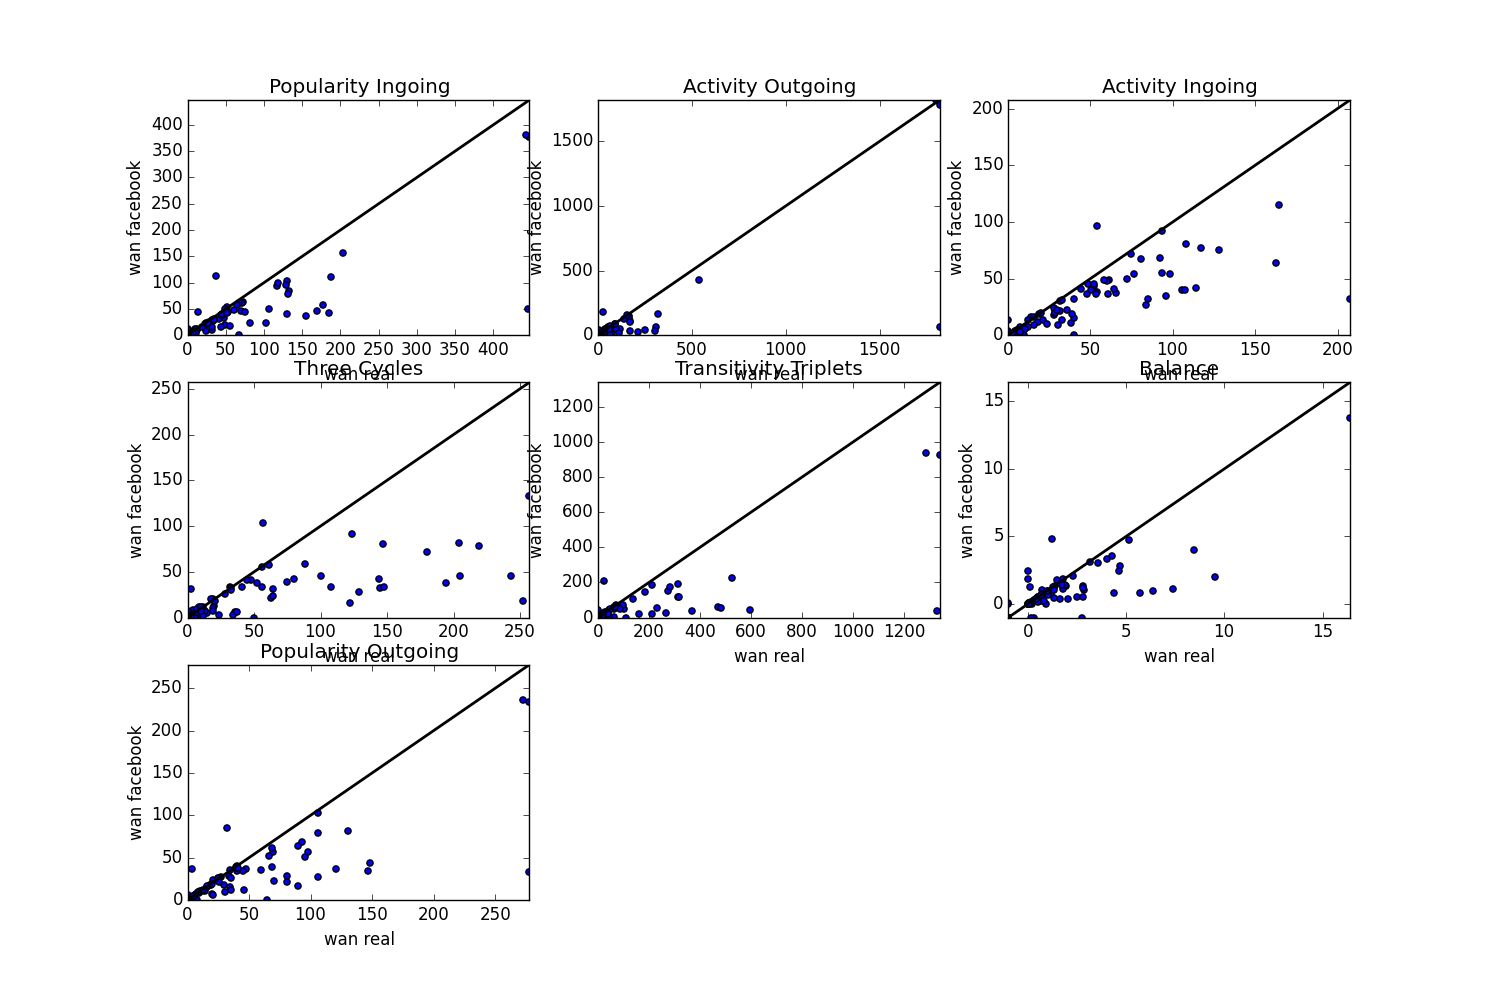
\includegraphics[scale=.55]{wan}
\caption{Comparison of node metrics on real VS facebook WAN}
\end{figure*}

\begin{figure*}[!htb]
\centering
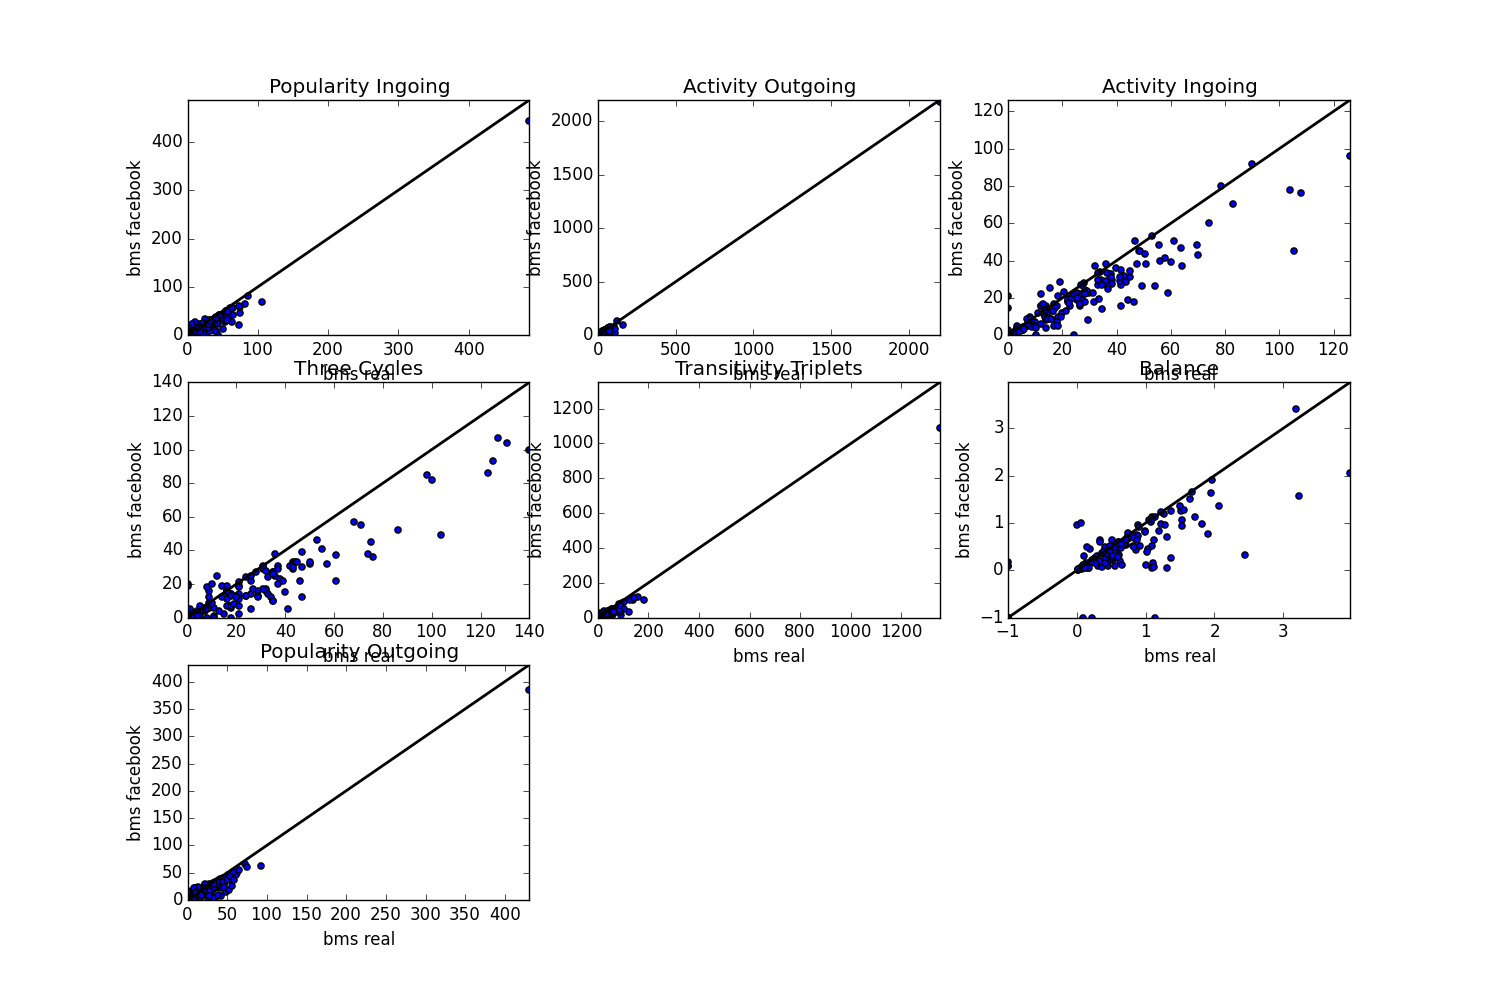
\includegraphics[scale=.55]{bms}
\caption{Comparison of node metrics on real VS facebook BMS}
\end{figure*}

% that's all folks
\end{document}


